\documentclass[12pt, a4paper, oneside]{article}

\usepackage{fontspec}
\usepackage[polish]{babel}
\usepackage{geometry}
\usepackage{graphicx}
\usepackage{booktabs}
\usepackage{array}
\usepackage{longtable}
\usepackage{hyperref}
\usepackage{float}
\usepackage{enumitem}
\usepackage{xcolor}
\usepackage{listings}

\geometry{margin=2.5cm}

\definecolor{codebg}{RGB}{245,245,245}
\definecolor{codekw}{RGB}{0,90,170}

\lstset{
    basicstyle=\ttfamily\footnotesize,
    backgroundcolor=\color{codebg},
    keywordstyle=\color{codekw}\bfseries,
    breaklines=true,
    columns=fullflexible,
    frame=single,
    framesep=4pt,
    rulecolor=\color{black!20},
    showstringspaces=false
}

\hypersetup{
    colorlinks=true,
    linkcolor=blue!60!black,
    urlcolor=blue!60!black,
    pdftitle={Kamień Milowy II -- Implementacja systemu},
    pdfauthor={Bartłomiej Karkoszka, Rafał Grot, Filip Stępień}
}

\title{\LARGE\bfseries Kamień Milowy II -- Implementacja systemu\\[0.8cm]
  {\Large Aplikacja do zarządzania zadaniami}}
\author{Bartłomiej Karkoszka \and Rafał Grot \and Filip Stępień}
\date{Przedmiot: Modelowanie i Analiza Systemów Informatycznych\\Grupa: 1ID21A}

\raggedbottom

\sloppy
\emergencystretch=3em

\begin{document}

% ============================================================
% STRONA TYTUŁOWA
% ============================================================
\maketitle
\thispagestyle{empty}

\vspace{1.0cm}

\tableofcontents
\newpage

% ============================================================
% 1. WPROWADZENIE
% ============================================================
\section{Wprowadzenie}

Niniejszy dokument stanowi raport z~drugiego kamienia milowego projektu \emph{Aplikacja do zarządzania zadaniami}. Etap ten obejmuje:
\begin{itemize}
  \item implementację podstawowych funkcjonalności systemu (REST API, persystencja, autoryzacja, interfejs użytkownika),
  \item przygotowanie diagramu sekwencji dla wybranego scenariusza,
  \item przygotowanie diagramu aktywności dla wybranego procesu systemowego,
  \item aktualizację wcześniej wykonanych diagramów (przypadków użycia, klas, komponentów oraz warstw) zgodnie z~rzeczywistą implementacją.
\end{itemize}

W~stosunku do pierwszego kamienia milowego nastąpiła istotna zmiana stosu technologicznego po stronie backendu -- początkowo planowany Spring Boot (Java) został zastąpiony przez \textbf{Go} z~routerem \texttt{chi} oraz generatorem kodu \texttt{sqlc}. Decyzja była motywowana chęcią wypróbowania języka Go w~praktyce.

% ============================================================
% 2. STAN IMPLEMENTACJI
% ============================================================
\section{Stan implementacji}

\subsection{Struktura repozytorium}
Projekt zorganizowany jest jako monorepo zawierające dwie aplikacje:
\begin{itemize}
  \item \texttt{apps/task-api} -- backend w~Go (REST API),
  \item \texttt{apps/task-frontend} -- frontend w~React 19 (SPA),
\end{itemize}
oraz konfigurację infrastruktury (\texttt{docker-compose.yml}, \texttt{docker/keycloak/realm.json}, \texttt{flake.nix}).

\subsection{Funkcjonalności zaimplementowane}

\begin{itemize}
  \item \textbf{Uwierzytelnianie i~autoryzacja} -- middleware HTTP weryfikujący tokeny JWT przy użyciu kluczy publicznych pobieranych z~serwisu Keycloak (JWKS). Pierwsze żądanie nowego użytkownika powoduje automatyczną synchronizację profilu (utworzenie wpisu w~tabeli \texttt{users} na podstawie pól \texttt{sub}, \texttt{name}, \texttt{email} z~tokenu).
  \item \textbf{Zarządzanie zadaniami (CRUD)} -- pełen zestaw operacji \texttt{POST}, \texttt{GET}, \texttt{PUT}, \texttt{DELETE} na zasobie zadań, zagnieżdżonym pod identyfikatorem użytkownika.
  \item \textbf{Filtrowanie listy zadań} -- parametry zapytania \texttt{status} oraz \texttt{priority} są walidowane i~przekazywane do dedykowanych zapytań SQL.
  \item \textbf{Dashboard} -- agregujący endpoint zliczający zadania zgrupowane po statusie (\texttt{todo}, \texttt{in\_progress}, \texttt{done}) oraz całkowitą liczbę zadań.
  \item \textbf{Walidacja danych wejściowych} -- DTO posiadają metody \texttt{Validate()} sprawdzające obecność tytułu, dopuszczalne wartości statusu i~priorytetu oraz format daty (\texttt{YYYY-MM-DD}).
  \item \textbf{Dokumentacja API} -- automatycznie generowana specyfikacja OpenAPI / Swagger UI dostępna pod ścieżką \texttt{/swagger}, z~konfiguracją OAuth2/PKCE wskazującą na realm Keycloak.
  \item \textbf{Health check} -- endpoint \texttt{/health} weryfikujący dostępność bazy danych.
  \item \textbf{Frontend} -- responsywny interfejs zbudowany w~React 19, z~Redux Toolkit (\texttt{createEntityAdapter}, thunki), komponentami z~biblioteki shadcn/ui i~stylowaniem Tailwind CSS v4. Strona \texttt{TasksPage} prezentuje statystyki, listę zadań oraz dialog tworzenia.
  \item \textbf{Konteneryzacja} -- \texttt{docker-compose.yml} uruchamia PostgreSQL (osobne instancje dla aplikacji i~Keycloaka), Keycloak (z~importem realmu) oraz panel Adminer.
\end{itemize}

\subsection{Lista endpointów REST}
Wszystkie endpointy są zabezpieczone middleware \texttt{Protect} (wymagany nagłówek \texttt{Authorization: Bearer <JWT>}) i~udostępnione pod prefiksem \texttt{/api} (konfigurowalnym przez zmienną \texttt{API\_BASE\_PATH}).

\begingroup
\setlength{\tabcolsep}{4pt}
\renewcommand{\arraystretch}{1.15}
\begin{longtable}{@{}>{\raggedright\arraybackslash}p{1.6cm} >{\raggedright\arraybackslash\ttfamily\small}p{5.3cm} >{\raggedright\arraybackslash}p{4.6cm} >{\raggedright\arraybackslash}p{2.6cm}@{}}
\toprule
\textbf{Metoda} & \textbf{\normalfont\rmfamily Ścieżka} & \textbf{Opis} & \textbf{Kody} \\
\midrule
\endhead
GET    & /health                              & Stan aplikacji i~bazy danych & 200, 401, 500 \\
GET    & /users/\{userId\}/tasks              & Lista zadań użytkownika z~opcjonalnymi filtrami & 200, 400, 401, 500 \\
POST   & /users/\{userId\}/tasks              & Utworzenie nowego zadania & 201, 400, 401, 500 \\
GET    & /users/\{userId\}/tasks/\{id\}       & Szczegóły pojedynczego zadania & 200, 400, 401, 404, 500 \\
PUT    & /users/\{userId\}/tasks/\{id\}       & Aktualizacja zadania & 200, 400, 401, 404, 500 \\
DELETE & /users/\{userId\}/tasks/\{id\}       & Usunięcie zadania & 204, 400, 401, 404, 500 \\
GET    & /users/\{userId\}/dashboard          & Statystyki zadań użytkownika & 200, 400, 401, 500 \\
\bottomrule
\end{longtable}
\endgroup

\subsection{Schemat bazy danych}
Migracje (\texttt{goose}) tworzą tabele \texttt{users} oraz \texttt{tasks}, a~także typy wyliczeniowe \texttt{task\_status} (\texttt{todo}, \texttt{in\_progress}, \texttt{done}) i~\texttt{task\_priority} (\texttt{low}, \texttt{medium}, \texttt{high}). Tabela \texttt{tasks} posiada klucz obcy \texttt{user\_id} z~kaskadowym usuwaniem oraz znaczniki czasowe \texttt{created\_at}, \texttt{updated\_at}.

% ============================================================
% 3. STOS TECHNOLOGICZNY (AKTUALIZACJA)
% ============================================================
\section{Stos technologiczny -- aktualizacja}

\begin{itemize}
  \item \textbf{Frontend:} React 19, TypeScript, Vite 8, Tailwind CSS v4, shadcn/ui, React Router v7, Redux Toolkit, react-redux.
  \item \textbf{Backend:} Go (chi router, sqlc, goose, slog, swaggo).
  \item \textbf{Baza danych:} PostgreSQL 16.
  \item \textbf{Uwierzytelnianie:} Keycloak 26.2 (OAuth2 / OpenID Connect, PKCE, JWKS).
  \item \textbf{Konteneryzacja:} Docker, Docker Compose.
  \item \textbf{Środowisko deweloperskie:} Nix flake (\texttt{flake.nix}) oraz \texttt{Taskfile.yml}.
  \item \textbf{Kontrola wersji:} Git.
\end{itemize}

% ============================================================
% 4. ZAKTUALIZOWANE DIAGRAMY Z KAMIENIA I
% ============================================================
\section{Zaktualizowane diagramy z~kamienia I}

Wszystkie diagramy zostały dostosowane do rzeczywistej implementacji.

\subsection{Diagram przypadków użycia}
W~stosunku do wersji z~kamienia I dodany został przypadek \emph{Synchronizuj profil użytkownika}, włączany przez przypadek \emph{Zaloguj się} -- odpowiada on faktycznemu mechanizmowi tworzenia rekordu w~tabeli \texttt{users} przy pierwszym żądaniu autoryzowanym.

\begin{figure}[H]
  \centering
  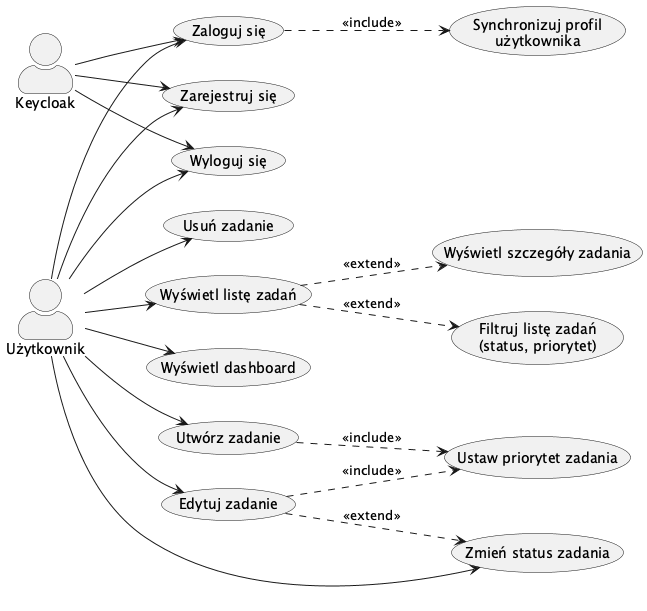
\includegraphics[width=0.9\textwidth]{diagrams/use_case_diagram.png}
  \caption{Diagram przypadków użycia}
\end{figure}

\subsection{Diagram klas}
Klasa \texttt{User} została rozszerzona o~pola \texttt{name}, \texttt{email}, \texttt{createdAt}, \texttt{updatedAt}, zgodnie z~migracją \texttt{00002\_add\_user\_profile\_columns.sql}. Klasa \texttt{Task} otrzymała pole \texttt{userId} (klucz obcy). Wartości typów wyliczeniowych dostosowano do nazw rzeczywistych (\texttt{todo}, \texttt{in\_progress}, \texttt{done}; \texttt{low}, \texttt{medium}, \texttt{high}). Dodano klasy pomocnicze \texttt{TaskFilters} oraz \texttt{DashboardSummary} odpowiadające DTO obecnym w~kodzie.

\begin{figure}[H]
  \centering
  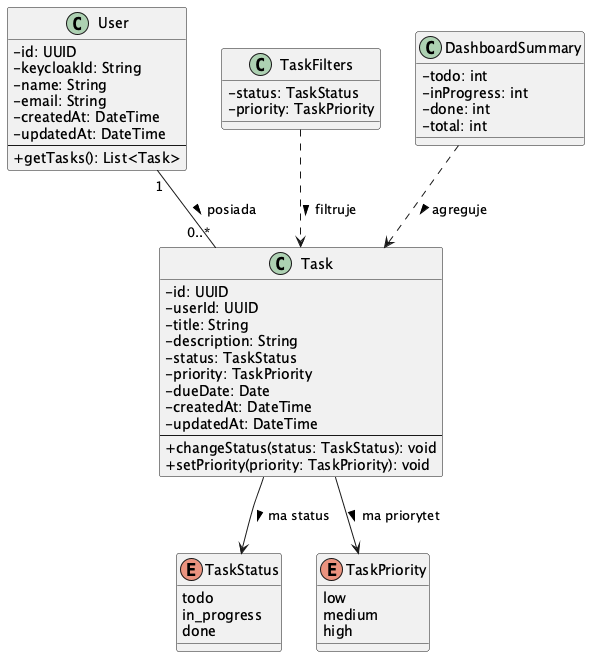
\includegraphics[width=0.85\textwidth]{diagrams/class_diagram.png}
  \caption{Diagram klas (model dziedziny + DTO)}
\end{figure}

\subsection{Diagram komponentów}
Diagram odzwierciedla rzeczywiste pakiety: po stronie frontendu wyodrębniono Redux Store (slice, thunki, selektory) oraz konkretne komponenty UI (\texttt{Layout}, \texttt{TaskDialog}, \texttt{TaskItem}, \texttt{StatCard}, \texttt{ProfileMenu}). Po stronie backendu przedstawiono router \texttt{chi}, \texttt{AuthMiddleware} z~weryfikacją JWKS, handlery \texttt{TaskHandler} i~\texttt{HealthHandler}, warstwę serwisów oraz wygenerowane przez \texttt{sqlc} \texttt{Queries}. Endpoint Swagger UI został wskazany jako osobny komponent.

\begin{figure}[H]
  \centering
  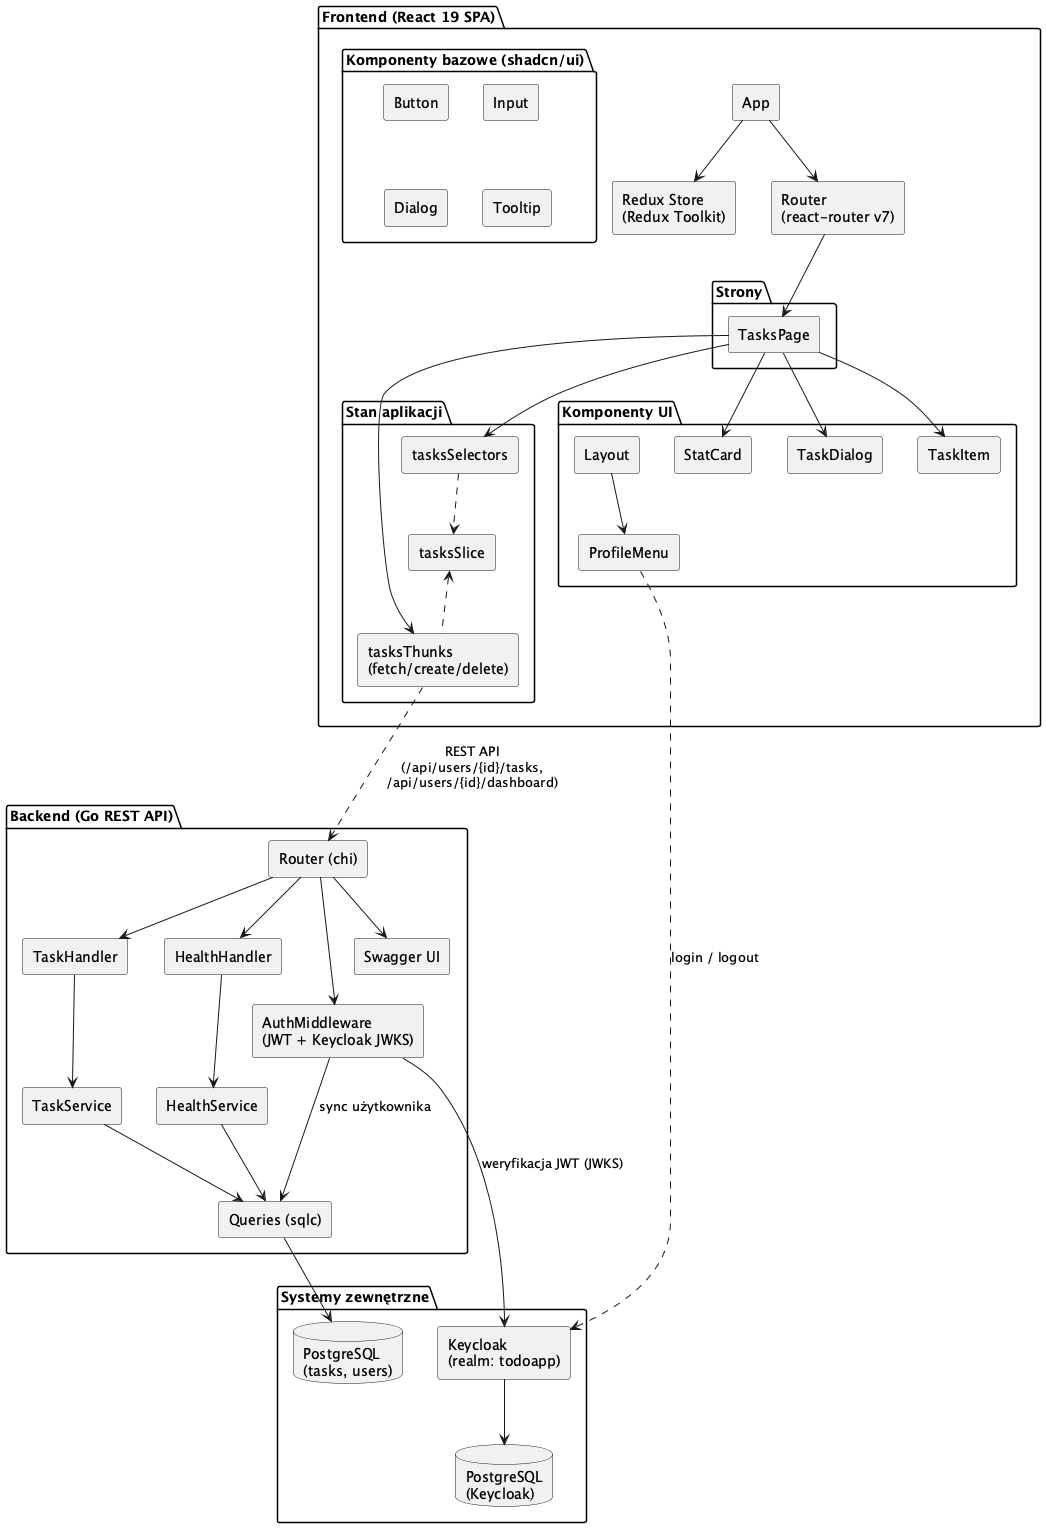
\includegraphics[width=\textwidth]{diagrams/component_diagram.png}
  \caption{Diagram komponentów}
\end{figure}

\subsection{Diagram warstw systemu}
Etykiety warstw zaktualizowano zgodnie z~zaimplementowanymi technologiami: warstwa prezentacji opisuje stack React 19 + Redux Toolkit, warstwa API -- chi i~Swagger UI, warstwa logiki -- handlery i~serwisy, warstwa dostępu do danych -- generowane przez \texttt{sqlc} zapytania, a~warstwa bezpieczeństwa -- middleware weryfikujący JWT.

\begin{figure}[H]
  \centering
  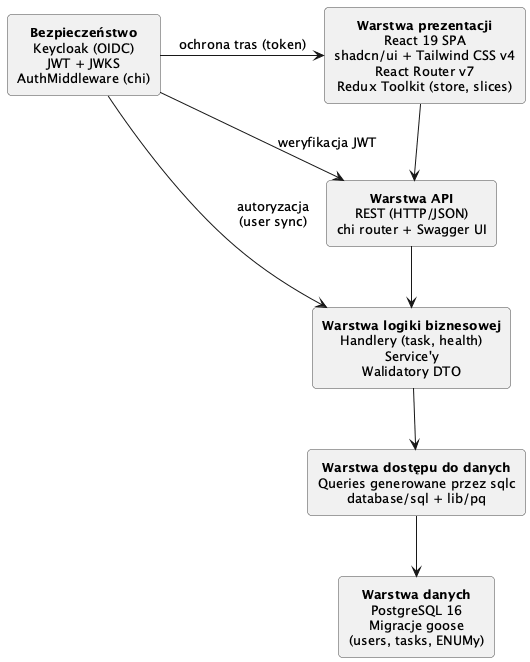
\includegraphics[width=0.78\textwidth]{diagrams/layer_diagram.png}
  \caption{Diagram warstw systemu}
\end{figure}

% ============================================================
% 5. DIAGRAM SEKWENCJI
% ============================================================
\section{Diagram sekwencji -- utworzenie zadania}

\textbf{Wybrany scenariusz:} użytkownik tworzy nowe zadanie. Scenariusz został wybrany, ponieważ ilustruje pełny przepływ przez wszystkie warstwy systemu -- od interakcji w~UI, przez akcję Redux i~żądanie HTTP, weryfikację tokenu, synchronizację użytkownika, walidację DTO, persystencję w~bazie, aż po aktualizację stanu po stronie klienta.

\begin{figure}[H]
  \centering
  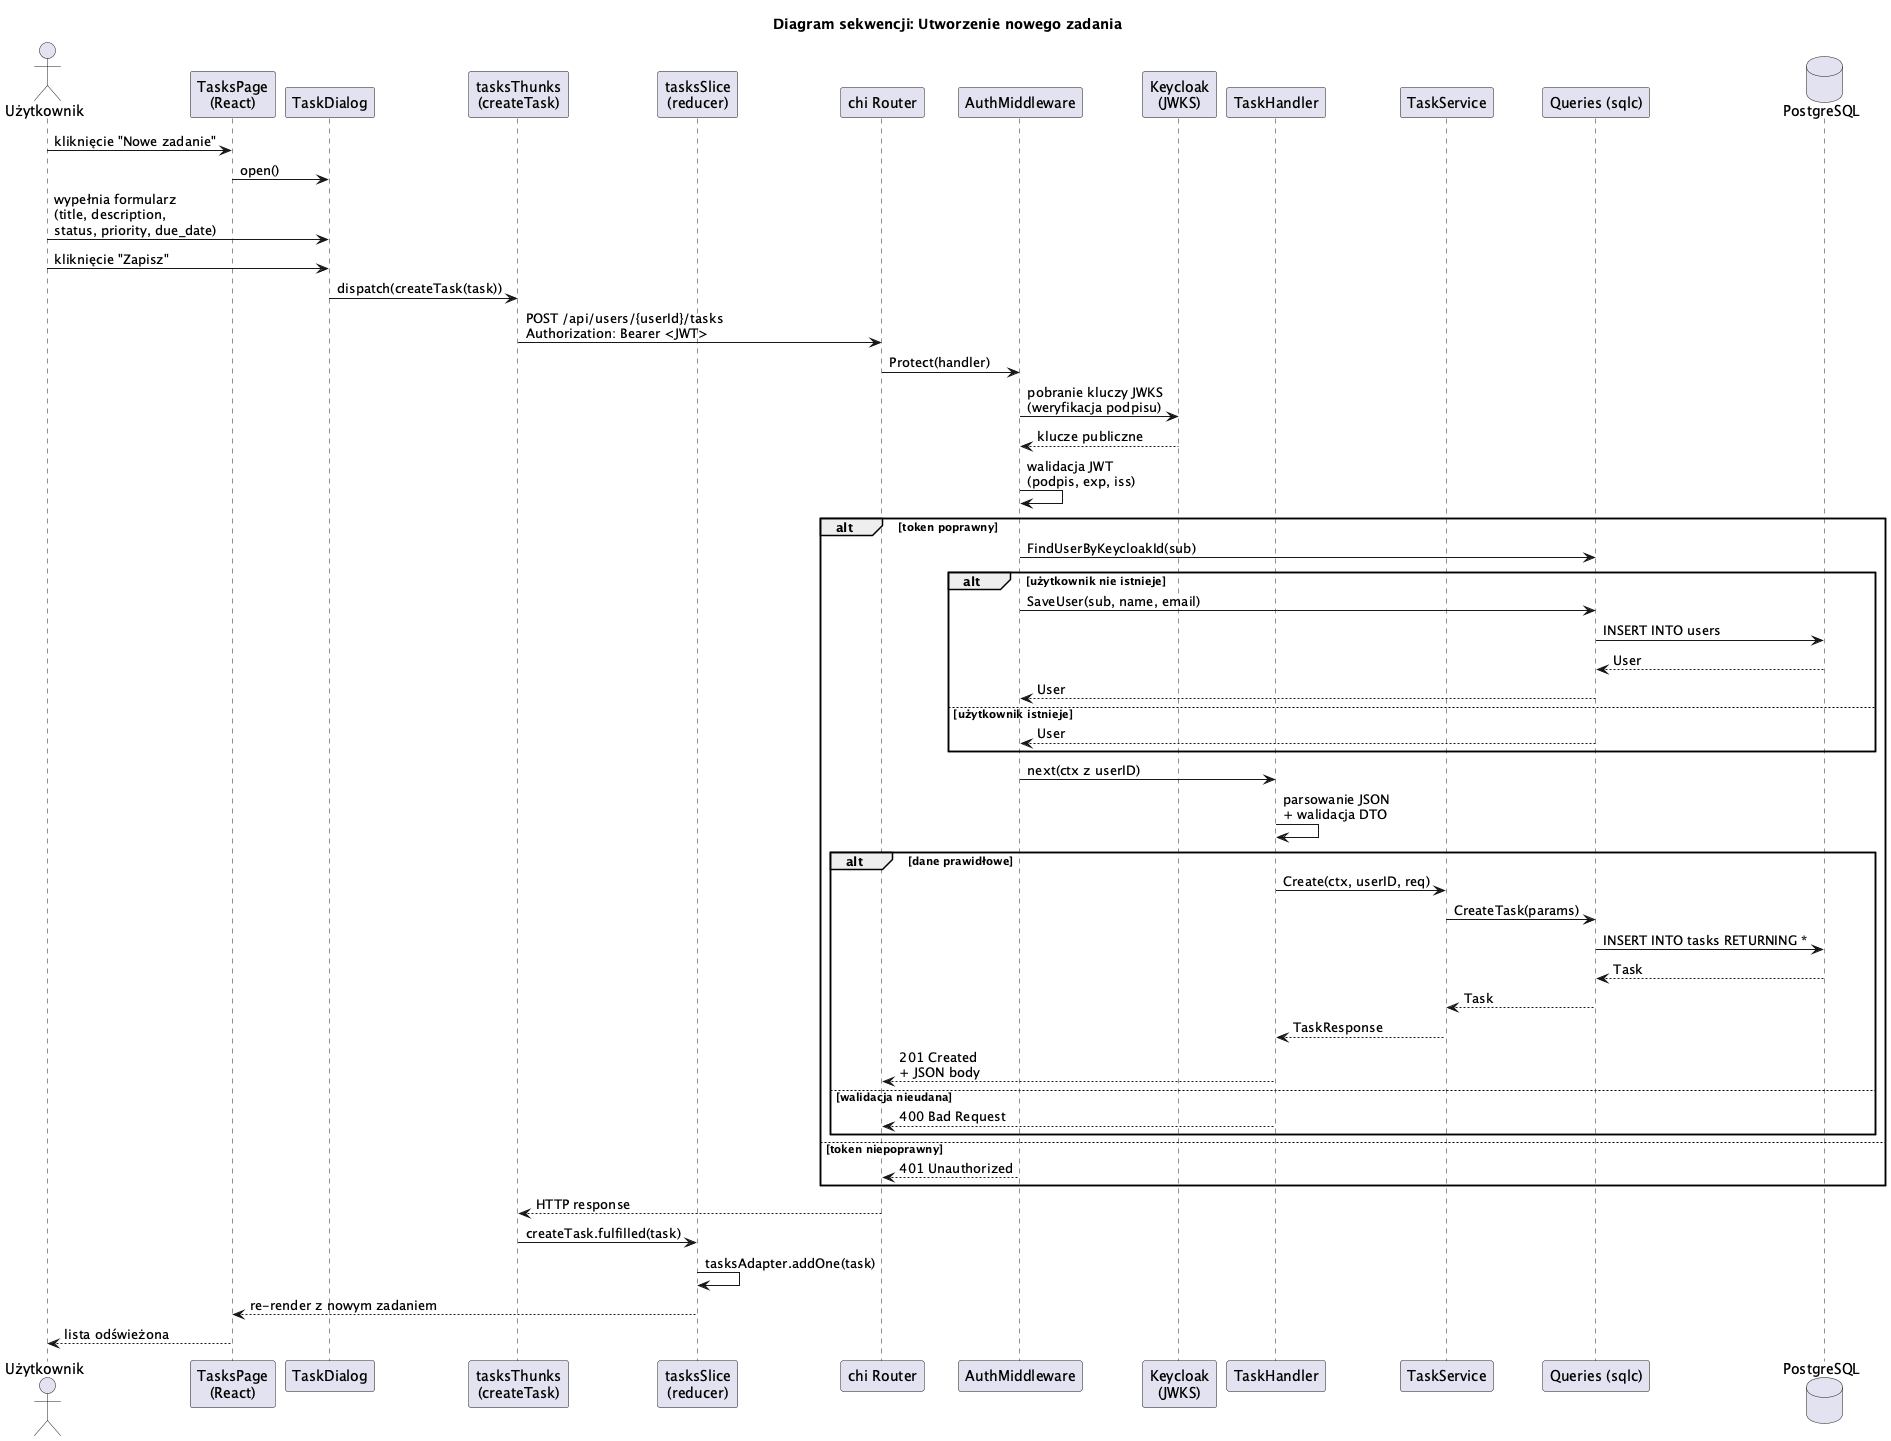
\includegraphics[width=\textwidth]{diagrams/sequence_diagram.png}
  \caption{Diagram sekwencji: utworzenie nowego zadania}
\end{figure}

\paragraph{Opis kluczowych kroków.}
\begin{enumerate}
  \item Użytkownik otwiera dialog \texttt{TaskDialog} ze strony \texttt{TasksPage} i~zatwierdza formularz.
  \item Frontend wywołuje thunk \texttt{createTask}, który wysyła żądanie \texttt{POST /api/users/\{userId\}/tasks} wraz z~tokenem JWT.
  \item \texttt{AuthMiddleware} pobiera klucze z~JWKS Keycloaka i~weryfikuje podpis tokenu.
  \item Jeżeli użytkownik o~podanym \texttt{sub} nie istnieje w~bazie, jest tworzony (synchronizacja profilu); w~przeciwnym wypadku rekord jest tylko odczytywany.
  \item \texttt{TaskHandler} parsuje ciało żądania, uruchamia \texttt{Validate()} na DTO, a~następnie wywołuje \texttt{TaskService.Create}.
  \item Serwis przekazuje parametry do wygenerowanego zapytania \texttt{CreateTask}, które wykonuje \texttt{INSERT INTO tasks RETURNING *}.
  \item Odpowiedź \texttt{201 Created} z~zserializowanym zasobem trafia do thunka, który wywołuje akcję \texttt{createTask.fulfilled} -- reducer dodaje encję do \texttt{tasksAdapter}, co skutkuje ponownym renderowaniem listy.
\end{enumerate}

% ============================================================
% 6. DIAGRAM AKTYWNOŚCI
% ============================================================
\section{Diagram aktywności -- zarządzanie zadaniem}

\textbf{Wybrany proces:} ogólna obsługa żądania zarządzania zadaniem (utworzenie, edycja, zmiana statusu, usunięcie). Diagram zawiera punkty decyzyjne dla wszystkich istotnych ścieżek błędu obecnych w~implementacji: 401 (brak/niepoprawny token), 400 (błędne dane wejściowe) oraz 404 (\texttt{sql.ErrNoRows}).

\begin{figure}[H]
  \centering
  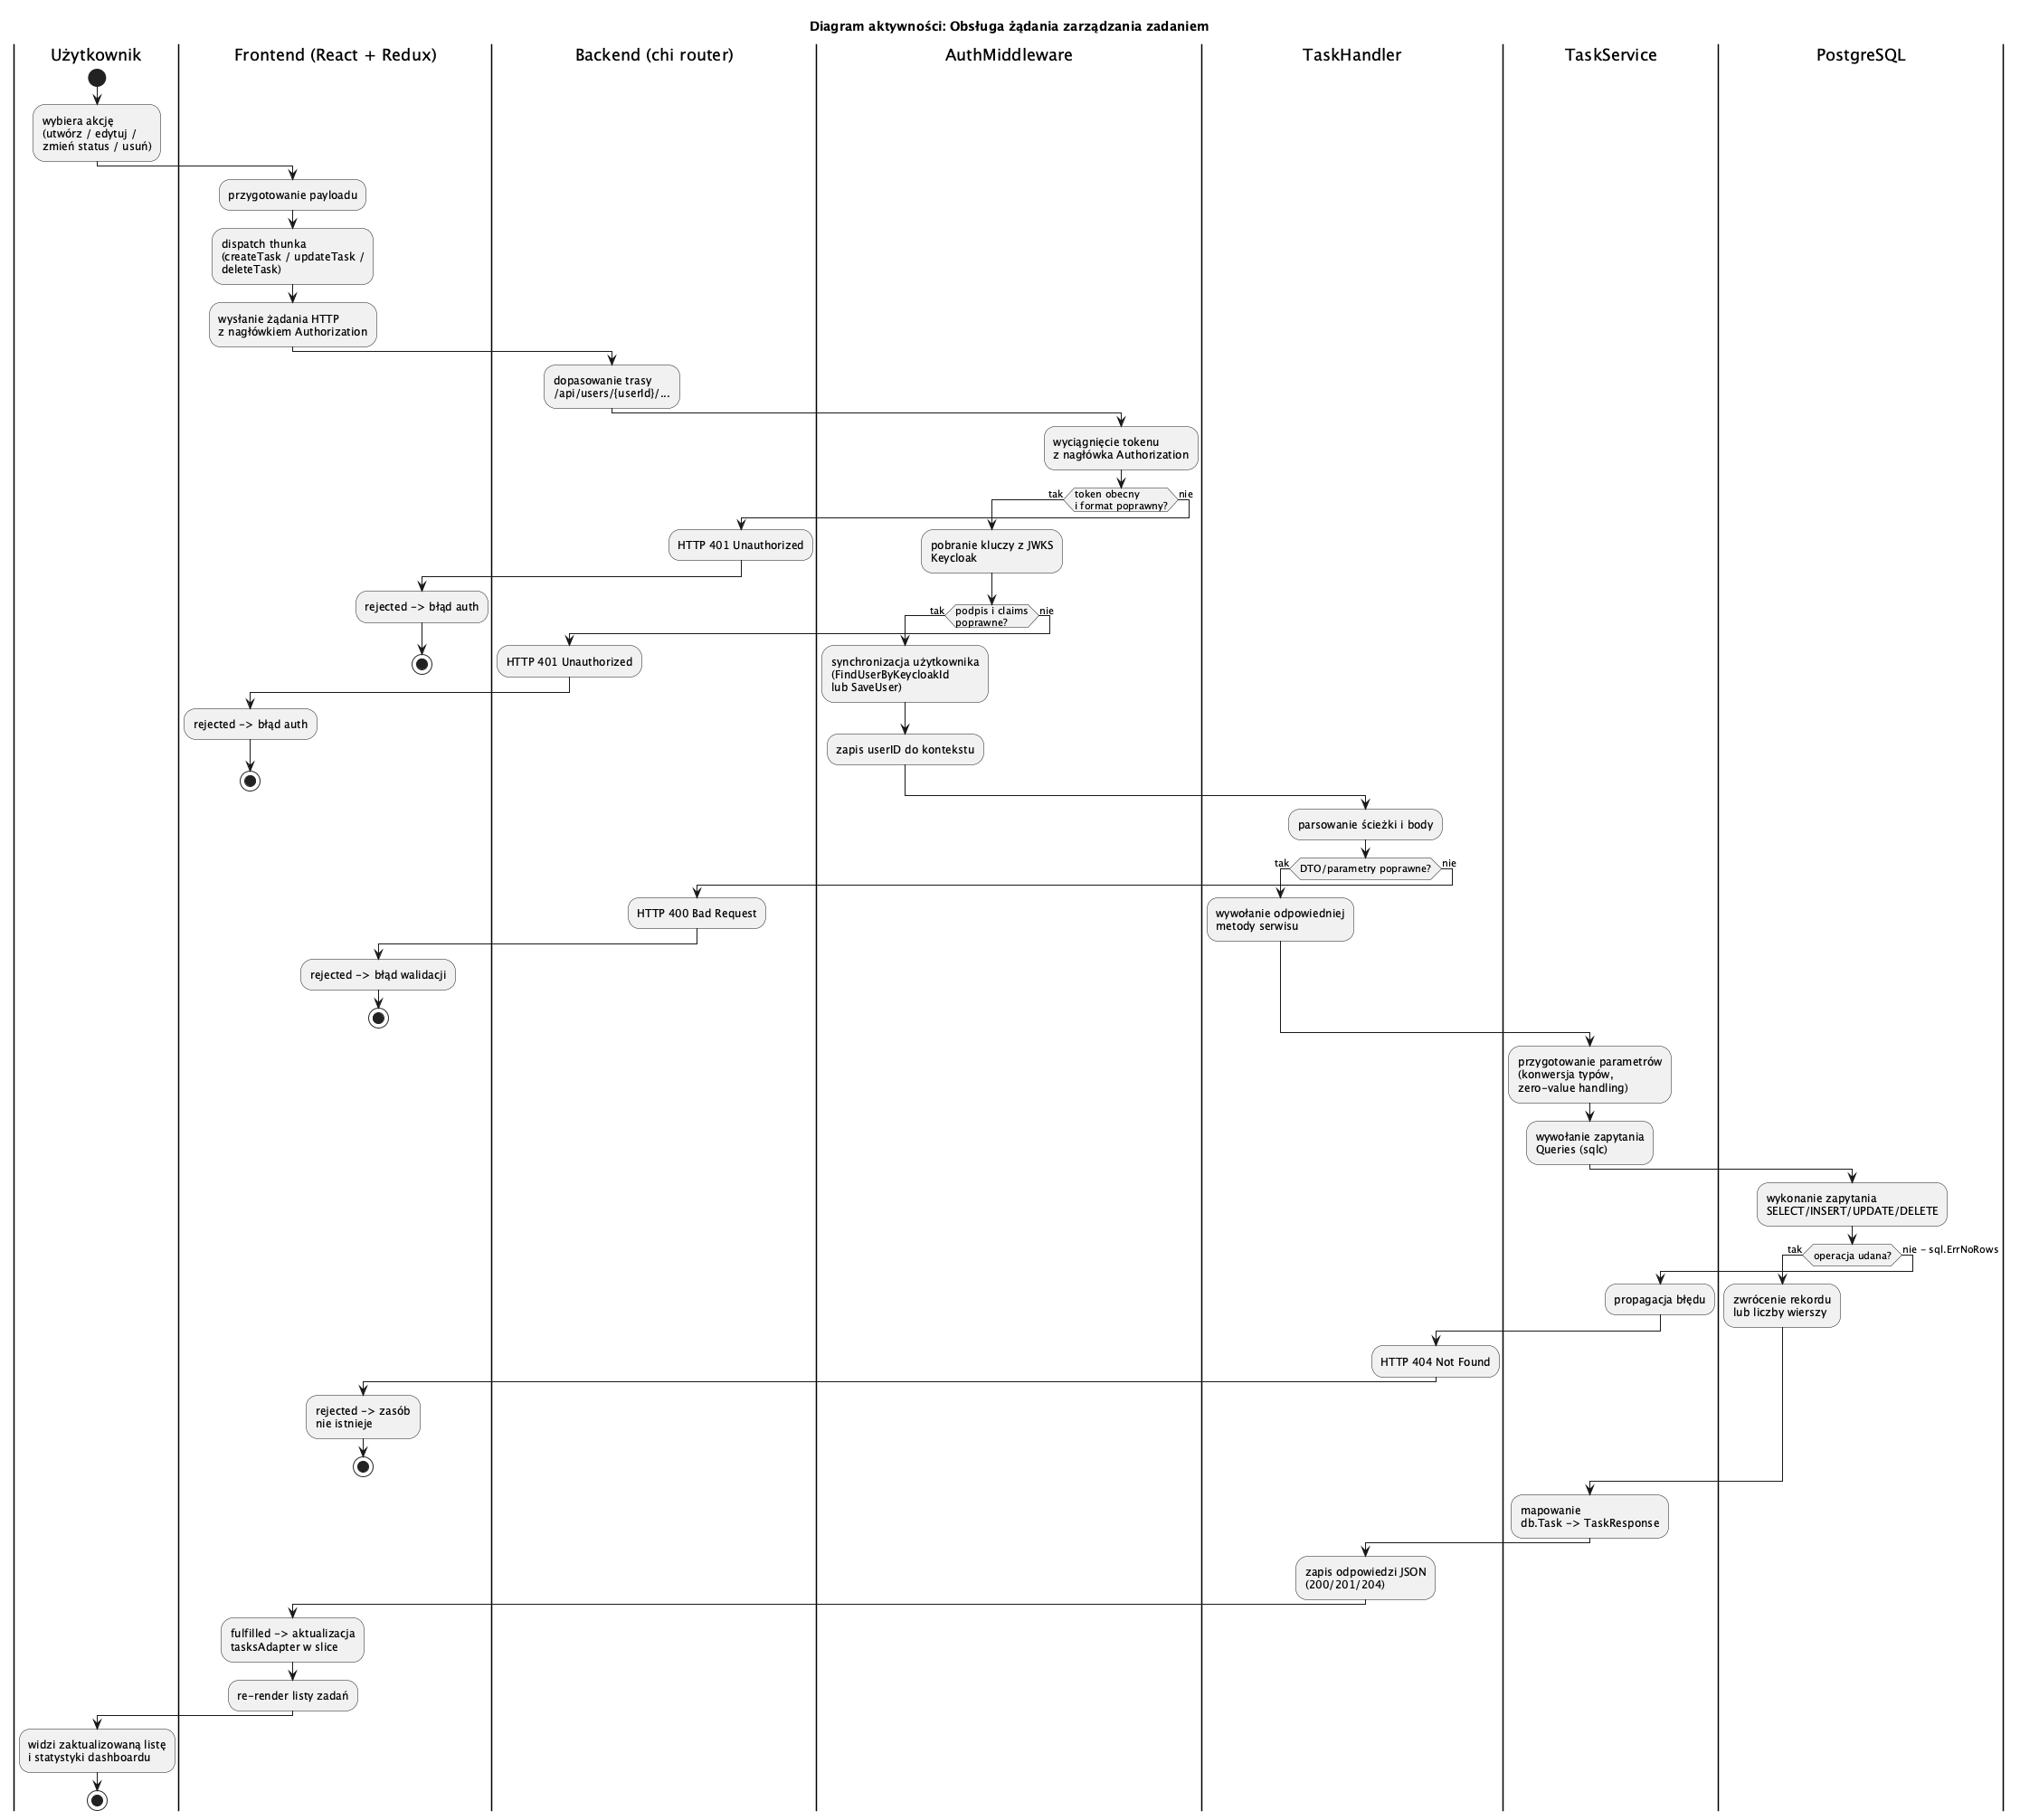
\includegraphics[width=\textwidth]{diagrams/activity_diagram.png}
  \caption{Diagram aktywności: obsługa żądania zarządzania zadaniem}
\end{figure}

\paragraph{Tory (swimlanes).}
Diagram wyodrębnia odpowiedzialności komponentów: \emph{Użytkownik}, \emph{Frontend (React + Redux)}, \emph{Backend (chi router)}, \emph{AuthMiddleware}, \emph{TaskHandler}, \emph{TaskService} oraz \emph{PostgreSQL}.

% ============================================================
% 7. URUCHAMIANIE I WERYFIKACJA
% ============================================================
\section{Uruchamianie i~weryfikacja}

\subsection{Wymagania wstępne}
Docker, Docker Compose, Go 1.22+, Node.js 20+ oraz \texttt{task} (Taskfile).

\subsection{Kroki uruchomienia}
\begin{enumerate}
  \item Skopiowanie pliku \texttt{.env.example} do \texttt{.env} i~uzupełnienie zmiennych.
  \item Start usług infrastrukturalnych: \texttt{docker compose up -d postgres postgres-keycloak keycloak adminer}.
  \item Wykonanie migracji bazy danych: \texttt{task migrate} (lub \texttt{goose}).
  \item Uruchomienie API: \texttt{task api:dev} (\texttt{go run ./cmd}).
  \item Uruchomienie frontendu: \texttt{npm run dev} w~katalogu \texttt{apps/task-frontend}.
\end{enumerate}

\subsection{Weryfikacja}
Po starcie systemu dostępne są:
\begin{itemize}
  \item Swagger UI -- \texttt{http://localhost:<API\_PORT>/swagger/index.html},
  \item panel Keycloak -- \texttt{http://localhost:8080},
  \item Adminer -- \texttt{http://localhost:8081},
  \item frontend -- \texttt{http://localhost:5173}.
\end{itemize}

% ============================================================
% 8. PODSUMOWANIE
% ============================================================
\section{Podsumowanie}

W~ramach drugiego kamienia milowego dostarczono działającą wersję systemu obejmującą podstawowe scenariusze użycia: uwierzytelnianie przez Keycloak, zarządzanie zadaniami (CRUD), filtrowanie oraz dashboard. Dokumentacja projektowa została rozszerzona o~dwa nowe diagramy (sekwencji oraz aktywności), a~wcześniej przygotowane diagramy zaktualizowano zgodnie z~rzeczywistą implementacją -- w~tym kluczową zmianą stosu backendowego (Go zamiast Spring Boot) oraz rozszerzonym modelem użytkownika.

\end{document}
